% !TEX root = ../../main.tex
% !TeX spellcheck = de_DE

\chapter{Implementierung}
Dieses Kapitel beinhaltet technische Details zur Umsetzung des GANs.
Die Details beinhalten allgemeinere Projektinformationen und vorgenommene Anpassungen zur Optimierung.

\section{Hardware}
Das spätere Training wird auf einer GeForce GTX 1070 \cite{gtx-1070} durchgeführt.
Die dazu korrespondierende Low-Level-APIs sind die von Nvidia entwickelten und bereits erwähnten Bibliotheken CUDA \cite{cuda-doc} und cuDNN \cite{cudnn-doc}.  

\section{Projekt}
Diese Sektion beinhaltet allgemeine Informationen zum Projekt.
Sie ist insbesondere an die Leser gerichtet, die den Code selbst ausführen oder bei sich einbinden wollen.

\subsection{Umgebung}
Für die Implementierung des GAN werden verschiedene Dependencies genutzt.
Diese sind alle im \textit{Pipfile} definiert und können mit \textit{pipenv install} installiert werden.
Im Gegensatz zu einen \textit{pip install} wird dabei zusätzlich ein Virtual Envirionment erzeugt.
Das Virtual Environment verhindert insbesondere Version Conflicts in Python.
\newline

Aufgrund der trivialen Installation des Projekts werden an dieser Stelle nur die wichtigsten Dependencies für Vergleiche genannt.
Dabei handelt es sich um Python 3.9, Tensorflow 2.6 und Keras 2.8.
Es ist anzumerken, dass Tensorflow mithilfe von CUDA optimiert wurde.
CUDA erlaubt die Ausführung der Trainings auf der GPU, was den Trainingsprozess stark beschleunigt.

\subsection{Konfiguration}
\label{chapter:configuration-hyperparams}
Für das Projekt existieren diverse Hyperparameter, wie zum Beispiel die Anzahl an Bildern pro Label oder auch die exakten Werte für Hyperparameter.
Alle Konfigurationen können innerhalb der Dateien \textit{configuration.py} und \textit{hyperparameters.py}  bearbeitet werden.
Je nach Hyperparameter müssen dann die Bilder erneut generiert werden.

\begin{figure}[H]
	\centering
	\subfloat[
		\centering 
		configuration.py
	]{{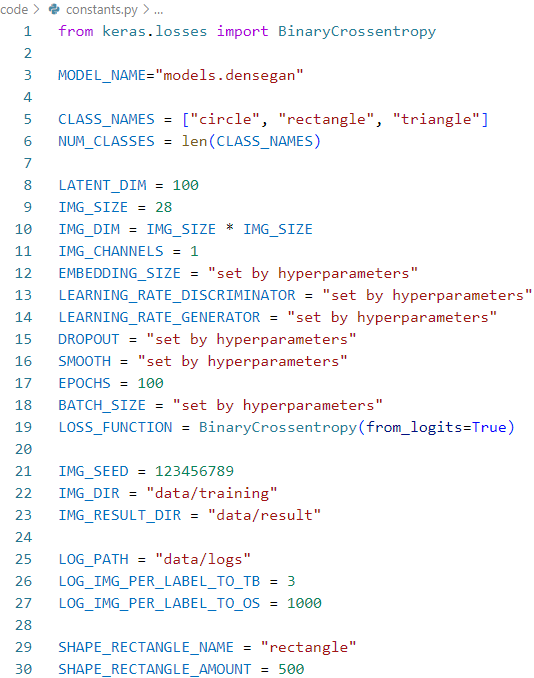
\includegraphics[height=8cm]{kapitel/4_implementierung/img/configuration.py.png} }}
	\qquad
	\subfloat[
		\centering 
		hyparameters.py
	]{{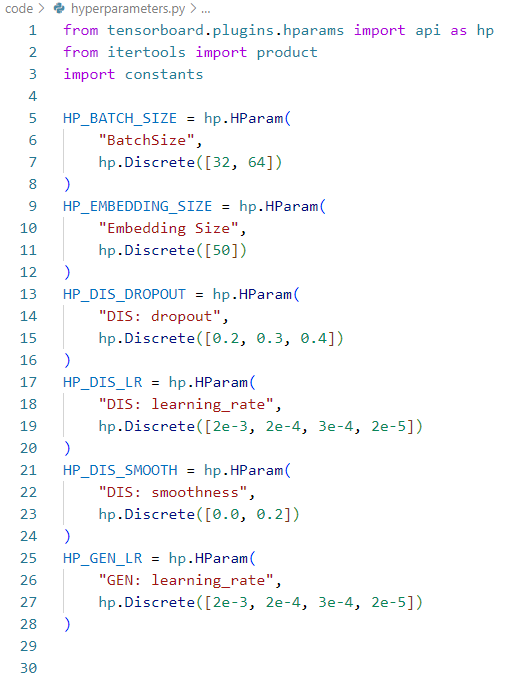
\includegraphics[height=8cm]{kapitel/4_implementierung/img/hyperparameters.py.png} }}
	\caption{Auszüge aus den Konfigurationsdateien}
	\label{imgs:config-hyperparams}
\end{figure}

Hyperparameter, die in der Datei \textit{configuration.py} als Wert den Text \textit{'set by hyperparameters'} haben, werden während des Trainings überschrieben.
Um die Hyperparameter zu ändern, muss die Datei \textit{hyperparameters.py} angepasst werden.
Gewünschte Hyperparameter können dort einfach in der entsprechenden Liste ergänzt werden.

\subsection{Ausführung}
Zunächst sollte der Model Name in der Datei \textit{constants.py} gesetzt werden.
Die Einstellung bestimmt das zu nutzende Modell.
Auch andere Hyperparameter können für das Training geändert werden (\cref{chapter:configuration-hyperparams}).
Falls zusätzlich zum Training eine Generierung stattfinden soll, muss in der Datei \textit{main.py} der Booleanwert \textit{GENERATE\_IMAGES} auf \textit{True} gesetzt werden.
Schließlich muss die Datei \textit{main.py} ausgeführt werden.
Das ausgeführte Script startet sowohl Generierungsprozess (falls konfiguriert) als auch das Training.

\subsection{Logs}
Bei den Logs handelt es sich um Bilder, FID-Werte und Graphen für die jeweilige Hyperparameterkombinationen.
Die Logs werden während dem Training automatisch erstellt.

Um die Logs einzusehen empfiehlt sich die Nutzung von Tensorboard.
Es sollte nach dem \textit{pip install} des \textit{Pipfile}s automatisch installiert sein.
Das Tensorboard kann mit dem Befehl \textit{tensorboard --logdir=data/logs/<model-name>} gestartet werden.

\section{Optimierungen}
Während der Arbeit wurden verschiedene Optimierungen vorgenommen, um entweder Ressourcen zu sparen oder den Trainingsprozess zu beschleunigen.
Die Optimierungen werden im Folgenden vorgestellt.

\subsection{Eigene Trainingsfunktion}
Tensorflow bietet eine Standardfunktion zum Traininieren von Neuronalen Netzen mit \textit{model.fit} an.
Die Funktion wird auf ein Model angewendet und führt eine Trainingsepoche auf einen übergebenen Datensatz mit zu übergebenden Parametern durch.
Die Funktion ist für simple Trainingsabläufe wie das Trainieren eines Klassifikatoren sehr gut geeignet.
Allerdings ist sie für den Trainingsablauf bei GANs ineffizient, da sie die beiden Modelle komplett separat trainiert.
\newline

Statt die Modelle einzeln zu trainieren, können die Losswerte von beiden Modellen verwendet werden.
Denn für einen Trainingsdurchlauf wird der Loss des Discriminators der echten und unechten Daten berechnet.
Der Discriminator benötigt für den Lernprozess beide Losswerte, der Generator nur den Loss des Discriminators für die unechten Daten.
Damit die Losswerte wiederverwendet werden können, wird eine eigene Trainingsfunktion benötigt.
Auf der Tensorflow Webseite ist dafür auch eine alternative Lernfunktion angegeben, die statt \textit{model.fit} verwendet wird \cite{tensorflow-gan-learn-step}.

\subsection{Matplotlib}
Für die Erstellung der Logs werden diverse Bilder erzeugt und abgespeichert.
Bei der Nutzung von Matplotlib muss dafür für jedes Bild zunächst eine Figur erstellt werden.
Die Figure wird benötigt, um das Bild zu konfigurieren.
Es ist dabei nicht möglich, die Figures für verschiedene Bilder vernünftig wiederzuverwenden.
\newline

Das Problem einer großen Anzahl an Figures ist, dass Matplotlib die Figures nicht automatisch bereinigt.
Stattdessen sammeln sich im Hintergrund immer mehr ungenutzte Objekte an.
Das führt zu einem ständig größer werdenden Arbeitsspeicherverbrauch.
Der erhöhte Verbrauch endet dann in einem Overflow Error und Absturz des Programms, in diesem Falle des Trainings.
\newline

Eine Lösung für das Löschen der Figure-Objekte ist die Methode \textit{plt.close('all')}, die von Matplotlib selbst bereitgestellt wird.
Sie löscht alle offenen Instanzen und bereinigt so den Arbeitsspeicher.
Die Methode muss jedoch manuell aufgerufen werden.
\newline

Um eine möglichst optimale Speichernutzung zu garantieren, wird die Funktion während des Trainings nach jedem geschriebenen Log ausgeführt.
Dadurch ist sichergestellt, dass auch lange Trainingsperioden durchgeführt werden können, ohne dass zusätzliche Ressourcen benötigt werden.

\subsection{Tensorflow-Keras}
Bei der Hyperparameteroptimierung werden verschiedene Modelle erzeugt und trainiert.
Tensorflow ist nicht dafür ausgelegt, in einem Durchgang sehr viele unterschiedliche Modelle zu trainieren.
Es existiert deshalb keine Automatismus, der nicht mehr benötigte Modell im Hintergrund aufräumt.
Dadurch kommt es zu einem stetig steigendem Arbeitsspeicher-Verbrauch.
\newline

Der Speicherverbrauch ist schlecht, da er zum Beispiel das Loggen verhindert.
Die entstehenden Probleme sind so gravierend, dass sie zu einem Abbruch des Lernprozesses führen können.
Die Lösung besteht im manuellen bereinigen der nicht mehr genutzten Modelle.
\newline

Für das Bereinigen stellt Tensorflow die Methode \textit{tf.keras.backend.clear\_session()} bereit.
Um eine möglichst optimale Speichernutzung zu gewährleisten wird die Methode nach jedem fertigen Model-Training aufgerufen.
So wird verhindert, dass Tensorflow gleichzeitig mehr als ein Modell bekannt ist.

\section{Daten-Generator}
Die Daten für das Training vom GAN sind synthetisch generiert mit einem eigens implementierten Generators.
Der Code für den Generator befindet sich in der Datei \textit{generator.py}.
Die Generierung der Bilder findet automatisch statt, sollte in der Datei \textit{main.py} der Boolean \textit{GENERATE\_IMAGES} auf True gesetzt sein.
\newline

Die Funktionen des Generators basieren auf dem Package skimage.
Bei dem Package handelt es sich um eine Sammlung von Methoden für Image-Processing und Computer Vision \todo{Quelle https://scikit-image.org/docs/dev/api/skimage.html}.
Insbesondere die Methoden zum Zeichnen von Polygonen und Kreisen werden zur Generierung angewendet.
\newline

Für die Generierung werden eine Bildgröße, Formmindestgröße, Formmaximalgröße und Anzahl zu generierender Bilder benötigt.
Die zugehörigen Werte sind in der Konfigurationsdatei \textit{constants.py} angegeben.

Beim Aufruf des Generators wird dann die jeweilige Generierungsfunktion für die Form aufgerufen.
Diese erstellt pro mögliche Größe eine Anzahl an Bildern.
Die Anzahl der Größen ist abhängig von der Anzahl der maximalen Bilder und berechnet sich mit der Formel: $AnzahlProGrö"se = MaximalAnzahlAnBildern / Grö"senKombinationen$.
\newline

Die Position der Form ist zufällig, kann aber durch einen Seed beeinflusst werden, um den Prozess reproduzieren zu können.
Durch die zufallsgesteuerte Positionierung können Positionen identisch sein.
Allerdings sind gleiche Bilder bei den verwendeten Konfigurationen sehr selten. \todo{Analyse gibt es gleiche Bilder?}

